%\documentclass[letterpaper]{IEEEtran}
\documentclass[letterpaper, conference]{IEEEtran}      % Use this line for a4 paper

%LatexiDiff ignore tikz:
% $: latexdiff -c "PICTUREENV=(?:picture|tikzpicture|DIFnomarkup)[\w\d*@]*" old.tex new.tex > diff.tex

%\IEEEoverridecommandlockouts                              %

%\usepackage{mathcomSTEP}

%\overrideIEEEmargins 
%\IEEEoverridecommandlockouts                              % This command is only needed if 
% you want to use the \thanks command

%\overrideIEEEmargins                                      % Needed to meet printer requirements.

% See the \addtolength command later in the file to balance the column lengths
% on the last page of the document

\onecolumn

\usepackage{mathptmx} 
\usepackage{times} 
\usepackage{amsmath} 
\usepackage{amsbsy} 
\usepackage{amssymb}
%\usepackage{newtxtext, newtxmath}
\usepackage{mathrsfs}
\usepackage{comment}
\usepackage[export]{adjustbox}
\usepackage{tikz}
\usetikzlibrary{external,positioning,decorations.pathreplacing,shapes,arrows,patterns}

%\tikzexternalize[mode=list and make]
\usepackage{algorithmicx}
\usepackage{pgfplots}
\usepackage{graphicx}
\usepackage{pstool}
\usepackage[latin1]{inputenc}
\usetikzlibrary{arrows,shapes}
\usepackage{xifthen}
\usepackage{epic}
\usepackage{caption}
\usepackage{epstopdf}

\newtheorem{thm}{\bf{Theorem}}
\newtheorem{cor}[thm]{\bf {Corollary}}
\newtheorem{lem}[thm]{\bf {Lemma}}
\newtheorem{prop}[thm]{\bf {Proposition}}
\newtheorem{example}{\bf {Example}}
\newtheorem{definition}{\bf {Definition}}
\newtheorem{rem}{\bf {Remark}}

\newcommand{\mmse}{\mathsf{mmse}}
\newcommand{\supp}{\mathrm{supp} }
\renewcommand\vec[1]{\ensuremath\boldsymbol{#1}}
\newenvironment{proof}{\paragraph*{Proof}}{\hfill$\square$ \newline}
\newcommand{\sgn}{\mathrm{sgn} }
\newcommand{\argmax}{\mathrm{argmax}}
\newcommand*{\QEDA}{\hfill\ensuremath{\square}}


\tikzstyle{int}=[draw, fill=blue!10, minimum height = 1cm, minimum width=1.5cm,thick ]
\tikzstyle{sint}=[draw, fill=blue!10, minimum height = 0.5cm, minimum width=0.8cm,thick ]
\tikzstyle{sum}=[circle, fill=blue!10, draw=black,line width=1pt,minimum size = 0.5cm, thick ]
\tikzstyle{ssum}=[circle, fill=blue!10,draw=black,line width=1pt,minimum size = 0.1cm]
\tikzstyle{int1}=[draw, fill=blue!10, minimum height = 0.5cm, minimum width=1cm,thick ]
\tikzstyle{enc}=[draw, fill=blue!10, minimum height = 2.7cm, minimum width=1cm,thick ]
\tikzstyle{int}=[draw, fill=blue!10, minimum height = 1cm, minimum width=1.5cm,thick ]


\title{\LARGE \bf Mean Estimation from Single-bit Measurements}
%
%\author{
%\IEEEauthorblockN{Alon Kipnis}
%\IEEEauthorblockA{Department of Electrical Engineering \\
%Stanford University\\
%Stanford, CA\\}
%\and
%\IEEEauthorblockN{John C. Duchi}
%\IEEEauthorblockA{Department of Statistics \\
%and Department of Electrical Engineering \\
%Stanford University\\
%Stanford, CA\\}
%\and
%\IEEEauthorblockN{Andrea J. Goldsmith}
%\IEEEauthorblockA{Department of Electrical Engineering \\
%Stanford University\\
%Stanford, CA\\}
%}

\begin{document}
\graphicspath{{../Figures/}}
\maketitle
\thispagestyle{empty}
\pagestyle{empty}



%%%%%%%%%%%%%%%%%%%%%%%%%%%%%%%%%%%%%%%%%%%%%%%%%%%%%%%%%%%%%%%%%%%%%%%%%%%%%%%%
\begin{abstract}
We consider the problem of estimating the mean of a normal distribution under the constraint that only a single bit per sample from this distribution is available to the estimator. We study the mean squared error risk in this estimation as a function of the number of samples, and hence number of bits, from this distribution. We consider an adaptive scheme in which each bit is a function of the current sample and the previously observed bits, as well as a fully distributed setting in which each bit is only a function of the current sample. For the adaptive scheme, we show that the optimal relative efficiency, compared to the standard mean estimator without bit limitation, is $\pi/2$. Namely, the number of samples required to attain the mean to a prescribed accuracy is only $\pi/2$ times larger due to the bit constraint. For the distributed scheme we consider the setting where each bit is obtained by comparing the current sample to a prescribed value. For this setting, we show that the expected asymptotic efficiency converges to $\pi/2$ provided that the variance of the distribution is high compared to the apriori uncertainty about the mean. Our results indicate that, rather surprisingly, parametric estimation from the coarsest form of quantization without significant penalty in the number of measurements is possible. 
\end{abstract}

%{\color{red}  The $\mu$-sum problem (Kim-ElGamal Ch. 21) gives a lower bound. Can be reduced to the CEO.}

%{\color{red}  See LASSO results in http://arxiv.org/abs/1506.02181v1}

%%%%%%%%%%%%%%%%%%%%%%%%%%%%%%%%%%%%%%%%%%%%%%%%%%%%%%%%%%%%%%%%%%%%%%%%%%%%%%%%
\section{Background}
\label{sec:Intro}
Processing information on multiple physical locations may impose communication constraints on the amount of information that can be shared among different units of the system. 
%For example, emerging sensor network technologies in medicine and ``smart cities" use many low-cost sensors to collect large amounts of data and transmit it to remote locations. These sensors must operate under severe power restrictions, hence they are limited by their communication bandwidth. 
%For example, this constraint occurs in large-scale sensor arrays where information is collected at multiple physical locations and transmitted to a central estimation unit. 
In this situation, the ability to estimate a particular parameter is dictated not only by quality of observations but also by the constraint on the communication rate of the sensor, which may be severely restricted due to power, bandwidth, or size of data. The question that we ask is to what extent a parametric estimation task is affected by such communication constraints, and what are the fundamental performance of estimation subject to these restrictions. \\

In this paper we provide a precise answer to this question in a limited setting: the estimation of the mean $\theta$ of a normal distribution with a known variance $\sigma^2$, under the constraint that only a single bit can be communicated to the estimator on each sample from this distribution. As it turns out, the ability to share information before communicating it dramatically affects the performance in recovering $\theta$. We distinguish in particular among three different settings:
 \begin{itemize}
 \item[(i)] \emph{Centralized} encoding: all the $n$ encoders confer and produce a single $n$ bit message. 
 \item[(ii)] \emph{Adaptive} or \emph{sequential} encoding: the $i$th encoder observes the $i$th sample and the $i-1$ previously encoded observations.
 \item[(iii)] \emph{Distributed} encoding: the output of the $i$th encoder is only a function of the $i$th observation.
 \end{itemize}
As far as information sharing is concerned, it is evident that settings (iii) is a more restrictive version of (ii) which is more restrictive than (i). We are concerned with the mean squared error (MSE) risk in estimating $\theta$ as the number of observations $n$ goes to infinity. In particular, we are interested in the \emph{relative efficiency} of estimators in settings (i)-(iii), defined as the ratio between their MSE to $\sigma^2/n$. The latter is the MSE attained by the sample mean, which is the minimal risk estimator when no constraints on the communication are imposed. \par
%
It is well known that the relative efficiency in setting (i) is $1$ \cite{720540, zhang2013information, zhang1988estimation}, i.e., asymptotically, there is no loss in performance due to the communication constraint in this setting. Indeed, under setting (i) the sample mean can be described with an error exponentially decaying in $n$, leading to MSE of $\sigma^2/n + o(n)$. In this work we show that a similar result does not hold even in setting (ii): the relative efficiency of any adaptive estimator is at least $\pi/2$. Namely, a single bit per sample communication constraint in the adaptive setting incurs a minimal penalty of at least $\pi/2 \approx 1.57$ compared to an unconstrained estimator, or to the optimal estimator in setting (i). In addition to this negative statement, we provide an estimator which asymptotically attains this minimal relative efficiency, i.e., we show that this lower bound is tight. Moreover, we show that even in the distributed setting (iii), a relative efficiency of $\pi/2$ is possible as long as $\sigma^2$ is large compared to the variance of the prior distribution on $\theta$. These results are quite surprising since they show that, even under the coarsest form of quantization, an estimator based on $ \approx 1.59 n$ measurements achieves accuracy in MSE or confidence interval comparable to an estimator that uses $n$ samples with infinite bit-precision.  \par
%
%One clue for this surprising results is given in a famous problem in information theory denoted as the CEO problem, first presented by Berger et. al. in \cite{berger1996ceo}. In this problem, a firms CEO is required to estimate a signal  from information sent to it by multiple agents, where the $i$th agents is given a noisy observation of this signal and has a limited number of bits, say $R_i$, to describe its observation to the CEO. 


\subsection*{Related Works}
%\subsubsection*{Statistical inference under communication constraints}
Statistical inference problems under communication constraints were considered in information theory in 
\cite{han1987hypothesis, zhang1988estimation, 720540}. These works consider a multi-terminal source coding setting in which the $i$th terminal observes $n$ samples from the distribution and is allotted $nR_i$ bits to communicate its estimate. The main focus of these works is the difference between inference with communication constraint and the unconstrained vanilla statistical estimation setting, as the number of samples $n$ goes to infinity subject to a total finite rate constraint. Our setting (i) can be seen as a special case of this setting where with a single terminal and $R_1 = 1$.% whereas our case (iii) is obtained from this setting by taking $n=1$, $R_i=1$, and number of terminals grow with $n$. 
However, as explained in \cite[Sec. III]{720540}, a single terminal in this setting always lead to the unconstrained inference performance. Indeed, when all samples are taken from the same distribution, the \emph{type} of the sample \cite{csiszar1998method} is a sufficient statistics for any inference task, and the latter can be described using a number of codewords polynomial in $n$ regardless of the distribution of the samples. For this reason, attention is given in these works to inference problems involving multiple distributions observed at different locations and hence the results there do not apply to our setting. In fact, with a full access to the sample as in setting (i), the problem of encoding and estimating $\theta$ is reduced to the MSE attained by a scalar quantizer adjusted to the sufficient statistics of the sample. Finally, we note that setting (ii) includes as a special case the sigma-delta modulation (SDM) analog-to-digital conversion scheme with a constant input $\theta$ corrupted by Gaussian noise $Z_i$, as was considered in \cite{53738}. While it was shown there that the output of the modulator converges to the true constant input, the rate of this convergence was not analyzed and cannot be derived directly from the results of \cite{53738}. In fact, a corollary from the results in this paper we conclude that the rate of convergence of a SDM to a constant input signal is at most $\sigma^2\pi/2$ over the number of feedback iterations. Finally, the multiterminal source coding setting denoted as the CEO problem \cite{berger1996ceo} can be seen as a generalization of our setting (iii), where multiple draws of $\theta$ and rounds of $n$ bit communication is permitted. In particular, the minimal CEO distortion with $1$ bit per terminal provides a lower bound on the MSE risk.  \par
%The difference between this setting and ours is that in ours the parameter of interest is not an information source. By assuming a prior distribution on this parameter, the CEO provides a lower bound on the estimation error in the fully distributed setting (iii). This lower bound can be attained if we were to consider the average error in multiple independent realizations of our problem rather than a single realization as we do here. \\
%
%While our focus in this paper is on setting (ii), we note that unlike the above works, we are also interested in the optimal estimation performance for a finite number of observations and not only in their asymptotic behavior. 
%\subsubsection*{Relation to channel coding}
More related to our setting is the work \cite{zhang2013information} that considers the minimax MSE risk in estimating a vector of parameters from $m$ machines, where each machine has access to $n/m$ samples a limited number of bits to describe these samples. The main results of this work are lower bounds on the estimation error as a function of the total number of bits can be sent by each machine. In the terminology of \cite{zhang2013information}, our settings (ii) and (iii) fall under the category of \emph{interactive}, and  \emph{independent} communication protocols, respectively. %In both cases we use $m=n$ (single sample per machine) and communication constraint of a single bit per machine.
However, unlike in \cite{zhang2013information}, we focus on achievable schemes and tight bounds in $n$ for the asymptotic MSE risk, rather than its scaling rate. \\

The rest of this paper is organized as follows: the main problem is defined in Section~\ref{sec:problem}. Our main results are presented and discussed in Sections~ \ref{sec:sequential} and \ref{sec:distributed}. Concluding remarks are given in Section~\ref{sec:conclusions}.


%We also note that the counterpart of setting (iii) in the case of hypothesis testing was considered in \cite{52470}. 

%\subsubsection{Estimation from 1-bit measurements}
%Single-bit or binary detectors are the basis for digital technology, and works considers the estimation of parameters from the results of such detectors have been around from the early days of digital computing. The burst of works in compressed sensing in the previous decade also gave raise to multiple 1-bit results \cite{rice_university}. Due to the popularization of MIMO technology and the expected break of mm-wave in wireless communication there have been many works 1-bit detection at the A/D in the receiver \cite{2016arXiv160204193Z}. 



\section{Problem Formulation \label{sec:problem}}

\begin{figure}
\begin{center}
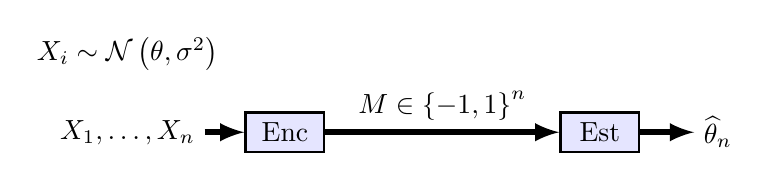
\begin{tikzpicture}[node distance=2cm,auto,>=latex]

\node[node distance = 1.5cm] at (0,0) (source2) {$X_1,\ldots,X_n$};
\node[int1, right of = source2, node distance = 2cm] (enc2) {Enc};  
\draw[->,line width = 2pt] (source2) -- (enc2); 

\node[above of = source2, node distance = 1cm] (dist) {$X_i \sim {\mathcal N} \left(\theta, \sigma^2 \right)$};

\node[int1, right of = enc2, node distance = 4cm ] (est) {Est};

\draw[->,line width = 2pt] (enc2) -- node[above, xshift = 0cm] (mes2) {$M \in \left\{-1,1\right\}^n$} (est);   

\node[right of = est, node distance = 1.5cm] (dest) {$\widehat{\theta}_n$};
%         \node [int1] (dec) [right of=dest, node distance = 1.5cm,  align=center] {\small Dec };
%\node [int1] (enc) [right of = dec, node distance = 3cm]{Enc}; 
%\draw[->,line width=2pt] (dec) -- (dest);
\draw[->, line width=2pt] (est) -- (dest);
\end{tikzpicture}
\end{center}
\caption{\label{fig:centralized} Centralized encoding using one bit per sample on average.}
\end{figure}


\begin{figure}
\begin{center}
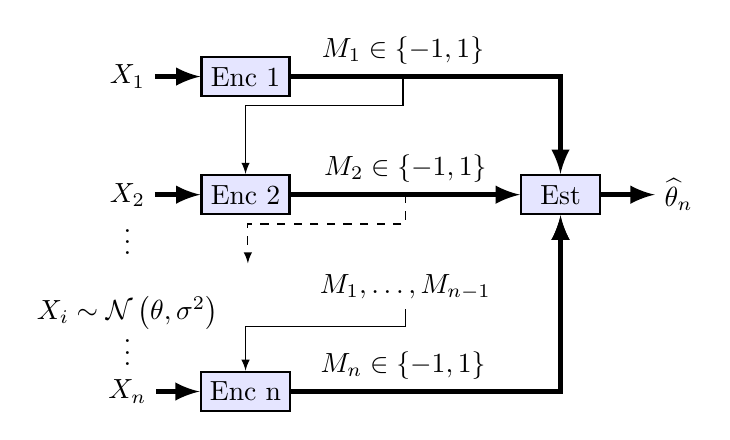
\begin{tikzpicture}[node distance=2cm,auto,>=latex]
  \node at (0,0) (source) {$X_1$} ;
  \node[int1, right of = source, node distance = 1.5cm] (enc1) {Enc 1};  
\draw[->,line width = 2pt] (source) -- (enc1); 

 \node[below of = source, node distance = 1.5cm] (source2) {$X_2$};
\node[int1, right of = source2, node distance = 1.5cm] (enc2) {Enc 2};  
\draw[->,line width = 2pt] (source2) -- (enc2); 

\node[below of = source2, node distance = 2.5cm] (source3) {$X_n$};
\node[int1, right of = source3, node distance = 1.5cm] (enc3) {Enc n};  
\draw[->,line width = 2pt] (source3) -- (enc3); 


\node[below of = source2, node distance = 0.5cm] {$\vdots$};
\node[above of = source3, node distance = 0.6cm] {$\vdots$};
\node[above of = source3, node distance = 1cm] (dist) {$X_i \sim {\mathcal N} \left(\theta, \sigma^2 \right)$};

\node[int1, right of = enc2, node distance = 4cm ] (est) {Est};
\draw[->,line width = 2pt] (enc1) -| node[above, xshift = -2cm] (mes1) {$M_1 \in \left\{-1,1\right\}$} (est);   
\draw[->,line width = 2pt] (enc2) -- node[above, xshift = 0cm] (mes2) {$M_2 \in \left\{-1,1\right\}$} (est);   
\draw[->] (mes1) -- +(0,-0.7) -| (enc2);

\draw[dashed,->] (mes2) -- +(0,-0.7) -| +(-2,-1.2);
\draw[->,line width = 2pt] (enc3) -| (est);   

\node[below of = mes2, node distance = 1.5cm] (mes3) {$M_1,\ldots,M_{n-1} $};

\draw[->,line width = 2pt] (enc3) -| node[above, xshift = -2cm]  {$M_n \in \left\{-1,1\right\}$} (est);   

\draw[->] (mes3) -- +(0,-0.5) -| (enc3);

\node[right of = est, node distance = 1.5cm] (dest) {$\widehat{\theta}_n$};
%         \node [int1] (dec) [right of=dest, node distance = 1.5cm,  align=center] {\small Dec };
%\node [int1] (enc) [right of = dec, node distance = 3cm]{Enc}; 
%\draw[->,line width=2pt] (dec) -- (dest);
\draw[->, line width=2pt] (est) -- (dest);
\end{tikzpicture}
\end{center}
\caption{\label{fig:sequential} Adaptive single-bit encoding: the $i$th encoder delivers a single bit message which is a function of its private sample $X_i$ and the previous messages $M_1,\ldots,M_{i-1}$.}
\end{figure}


\begin{figure}
\begin{center}
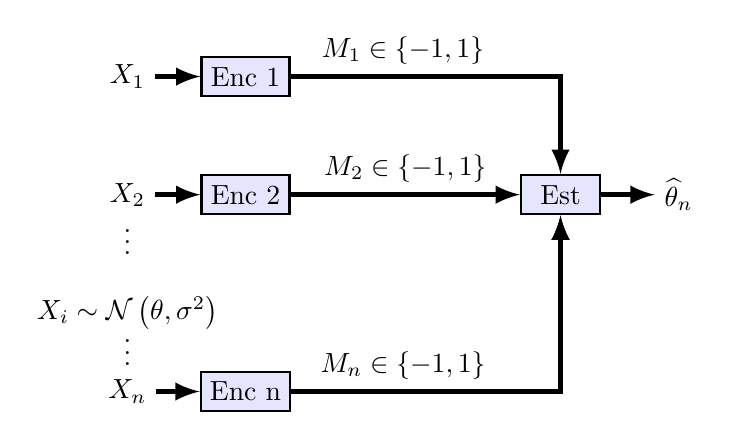
\begin{tikzpicture}[node distance=2cm,auto,>=latex]
  \node at (0,0) (source) {$X_1$} ;
  \node[int1, right of = source, node distance = 1.5cm] (enc1) {Enc 1};  
\draw[->,line width = 2pt] (source) -- (enc1); 

 \node[below of = source, node distance = 1.5cm] (source2) {$X_2$};
\node[int1, right of = source2, node distance = 1.5cm] (enc2) {Enc 2};  
\draw[->,line width = 2pt] (source2) -- (enc2); 

\node[below of = source2, node distance = 2.5cm] (source3) {$X_n$};
\node[int1, right of = source3, node distance = 1.5cm] (enc3) {Enc n};  
\draw[->,line width = 2pt] (source3) -- (enc3); 

\node[above of = source3, node distance = 1cm] (dist) {$X_i \sim {\mathcal N} \left(\theta, \sigma^2 \right)$};
\node[below of = source2, node distance = 0.5cm] {$\vdots$};
\node[above of = source3, node distance = 0.6cm] {$\vdots$};

\node[int1, right of = enc2, node distance = 4cm ] (est) {Est};
\draw[->,line width = 2pt] (enc1) -| node[above, xshift = -2cm] (mes1) {$M_1 \in \left\{-1,1\right\}$} (est);   

\draw[->,line width = 2pt] (enc2) -- node[above, xshift = 0cm] (mes2) {$M_2 \in \left\{-1,1\right\}$} (est);   

\draw[->,line width = 2pt] (enc3) -| (est);   

\draw[->,line width = 2pt] (enc3) -| node[above, xshift = -2cm]  {$M_n \in \left\{-1,1\right\}$} (est);   

\node[right of = est, node distance = 1.5cm] (dest) {$\widehat{\theta}_n$};
%         \node [int1] (dec) [right of=dest, node distance = 1.5cm,  align=center] {\small Dec };
%\node [int1] (enc) [right of = dec, node distance = 3cm]{Enc}; 
%\draw[->,line width=2pt] (dec) -- (dest);
\draw[->, line width=2pt] (est) -- (dest);
\end{tikzpicture}
\end{center}
\caption{\label{fig:distributed} Distributed single-bit encoding: the single-bit message produced by each encoder is only a function of its private sample $X_i$.}
\end{figure}


Let $X_i$, $i=1,\ldots,n$, be $n$ independent samples from the normal distribution $P(X) = \mathcal N(\theta,\sigma^2)$ with mean $\theta$ and variance $\sigma^2$. We also assume that the mean $\theta$ is drawn once from a prior distribution $\pi(\theta)$ on the parameter space $\Theta$, which is a closed interval of the real line. We moreover assume that $\pi(\theta)$ is absolutely continuous with respect to the Lebesgue measure with a bounded second moment. We denote the variance of $\theta$ with respect to $\pi(\theta)$ by $\sigma_\theta^2$. The problem we consider is the estimation of the parameter $\theta$ under the following constraints on the communication between the samples $X_1,\ldots,X_n$ and a centralized estimator: 
\begin{itemize}
\item[(i)] The estimator at time $n$ is only a function of the $n$ messages $M^n = \left(M_1,\ldots,M_n \right)$ (Fig.~\ref{fig:centralized}).
\item[(ii)] For each $i=1,\ldots,n$, the $i$th message $M_i$ is a function of the sample $X_i$ and the $i-1$ previous messages $M^{i-1}$ (Fig.~\ref{fig:sequential}).
\item[(iii)] The $i$th message $M_i$ takes only two possible values, say $1$ and $-1$ (Fig.~\ref{fig:distributed}).
\end{itemize}
In other words, the only information on the sample $X^n \left(X_1,\ldots,X_n\right)$ available to the estimator is the messages $M^n$. In addition, each message $M_i$ is a function from the real line into the set $\{-1,1\}$ which is measurable with respect to the sigma algebra generated by $M^{i-1}$ and $X_i$. The estimator, upon observing $M^n$, produces an estimate $\widehat{\theta}_n(M^n)$ of $\theta$. A system describing the above scheme is illustrated in Fig.~\ref{fig:sequential}. \\

The performance of this estimation is measured by the mean squared error (MSE) risk function:
\begin{equation}
\label{eq:error_def}
R_n \triangleq \mathbb E\left(\widehat{\theta}_n - \theta \right)^2,
\end{equation}
where the expectation is taken with respect to the distribution of $X^n$ and the prior distribution $\pi(\theta)$.  \\
%It is well known that minmax estimation error 
%\begin{equation}
%R_n = \min \sup_{\theta \in \Theta}  \mathbb E\left[ \left(\widehat{\theta}_n - \theta \right)^2 | \theta \right],
%\end{equation}
%can be obtained from $R_n$ by assuming a particular least favorable prior distribution on the parameter space $\Theta$ \cite{casella1981}. 

The main problem we consider is the minimal value that can be attain in \eqref{eq:error_def} as a function of $n$. Note that this minimization is the combination of the following two processes: (1) selecting the $i$th message $M_i$ based on past messages and current observation $X_i$, and (2) estimating $\theta$ given messages $M^n$. We are interested in particular in the asymptotic relative efficiency of estimators $\widehat{\theta}_n$ for $\theta$ compared to the sample mean $\bar{X}_n = \frac{1}{n} \sum_{i=1}^n X_i$. Since the MSE attained by the latter is $\sigma^2/n$, this relative efficiency is defined as
\begin{equation}
 \lim_{n \rightarrow \infty} \frac{n}{\sigma^2}  R_n. 
\label{eq:relative_efficiency}
\end{equation}
%{\color{red} Since the conditional expectation of $\theta$ with respect to $\bar{X}_n$ (and not $\bar{X}_n$) minimizes \eqref{eq:error_def}, we need to justify the fact that we use the sample mean as the reference estimator.}

In addition to the notations defined above, we denote by $\phi(x)$ the standard normal density and by $\Phi(x)$ the standard normal cumulative distribution function. Prime denote derivative with respect to $\theta$.


\section{Distributed Estimation \label{sec:distributed}}
We now consider the case where a single bit message is available on each sample from the distribution, and this message is independent of the other messages. Moreover, we assume that each message is characterized by a threshold value, and that ``$1$'' is sent by the $i$th encoder whenever $x_i$ is above this value. 

\subsection{Threshold Detection}
We assume that each message is of the form
\[
M_i = \sgn(t_i - X_i) = \begin{cases} 1 & X_i< t_i, \\
-1 & X_i > t_i,
\end{cases}  
\]
where $t_i\in\mathbb R$ is the \emph{threshold} of the $i$th detector applied by the encoder on it sample $X_i$. In order to characterize the asymptotic behavior of estimation from these sequence of messages, we consider the \emph{density} of $n$ threshold values defined as:
\[
\lambda_n([a,b]) = \frac{1}{n} \left| \mathcal T \cap [a,b] \right|,
\]
where $\mathcal T  = \left\{t_n, n \in \mathbb N \right\}$ is the collection of all threshold values. We further assume that $\lambda_n$ converges (weakly) to a probability measure $\lambda(t)$ on $\mathbb R$.  \par
In order to estimate $\theta$ from the messages $M^n$, we consider the maximum likelihood (ML) estimator. The log-likelihood function of $\theta$ is given by
\[
l(M^n  |\theta ) = \sigma  \sum_{i=1}^n \log \left( \Phi \left( M_i \frac{t_i - \theta}{\sigma} \right) \right). 
\]
Since $\Phi(x)$ is a log concave function, the log-likelihood function has a unique maximizer $\widehat{\theta}_n$ which is the ML estimator.  \\

Next, we show that under the assumptions above, the sequence of messages $M^n$ defines a local asymptotic normal (LAN) family of probability distributions. Therefore, the MSE in estimating $\theta$ from the messages $M^n$ satisfies a local asymptotic minimax property with respect to the \emph{precision} parameter of this LAN family \cite{van2000asymptotic}. Moreover, we conclude the ML estimator is locally asymptotic minimax. 

\begin{thm} \label{thm:LAN}
Consider the sequence of threshold detectors $M^n$ with threshold density converges to a probability measure $\lambda$. The the following two statements hold:
\begin{itemize}
\item[(i)] Any estimator ${\theta}_n$ of $\theta$ which is a function of $M^n$ satisfies
\[
\liminf_{c\rightarrow \infty}\, \liminf_{n\rightarrow \infty} \sup_{\tau\,:\,| \tau - \theta| \leq \frac{c}{\sqrt{n}} }  n \mathbb E \left({\theta}_n - \tau \right)^2 \geq \sigma^2/K(\theta),
\]
where 
\[
K(\theta) \triangleq \int \eta\left(\frac{t-\theta}{\sigma} \right) \lambda(dt),
\]
and 
\[
 \eta(x) = \frac{ \phi^2\left( x \right)}{ \Phi\left( x \right) \left(1-\Phi\left(x\right) \right)}. 
\]
\item[(ii)] The asymptotic distribution of the ML estimator $\widehat{\theta}_n$ is given by
\[
\sqrt{n}(\widehat{\theta}_n - \theta) \overset{D}{\rightarrow} \mathcal N\left(0,\sigma^2/K(\theta) \right).
\]
\end{itemize}
\end{thm}


\subsubsection*{Sketch of Proof}
The proof shows that the probability distribution of the vector of messages $M^n$ define a local asymptotic normal (LAN) family of probability distributions with precision parameter $K(\theta)/\sigma^2$. The statements in the theorem then follows from the local asymptotic minimax theorem of LAN families \cite{van2000asymptotic}. The details are given in the Appendix.\\


%Theorem~\ref{thm:dist_thresholds} shows that the maximum likelihood estimator of $\theta$ given the $n$ single-bit messages $M^n$ is asymptotically normal and attains the local asymptotic minimax error $\sigma^2/K(\theta)$. 

It follows from Thm.~\ref{thm:LAN} that the asymptotic risk of the ML estimator is $\sigma^2/K(\theta)$, and that this risk is asymptotically minimal over all local alternative estimators for $\theta$. Moreover, the relative efficiency of the ML in the threshold detection scheme equals $1/K(\theta)$. Since the thresholds density $\lambda(t)$ integrates to $1$, and from the bound on the function $\eta(x)$ obtained in the proof of Lemma~\ref{lem:bound_intervals}, it follows that
\[
K(\theta) \leq \sup_{t\in \mathbb R} \eta \left( \frac{t-\theta}{\sigma} \right) \int  \lambda(dt)  \leq \frac{2}{\pi}.
\]
This upper bound on $K(\theta)$ implies that the relative efficiency of any distributed estimator is at least $\pi/2$, a fact that agrees with the lower bound under adaptive estimation derived in Thm.~\ref{thm:adpative_lower_bound}. Unfortunately, this upper bound on $K(\theta)$ is attained whenever the density $\lambda$ is the mass distribution at $\theta$, which is unknown apriori. Therefore, in the section below we consider the asymptotic threshold density function $\lambda$ that minimize the expected asymptotic risk $\mathbb E\left [\sigma^2/K(\theta) \right]$. 


{\bf Worst case $\theta$}: in order to bound the local asymptotic minimax risk it is required to consider the desnity $\lambda$ that minimizes the worst case $\theta$ in the parameter space $\Theta$. We assume that $\Theta = [-b,b]$ for some $b>0$, and consider 
\begin{equation} \label{eq:variational}
\sup_{\lambda} \inf_{\theta \in [-b,b]}  {K(\theta)} = \int \eta\left( \frac{t-\theta}{\sigma} \right) \lambda (dt),
\end{equation}
where the suprimum is over all probability measure $\lambda$ on $\mathbb R$. Since \eqref{eq:variational} is concave in $\lambda$, this optimization problem can be solved using a convex program. 
As illustrated in Fig.~\ref{fig:cvx}, the threshold density that maximizes \eqref{eq:variational} is supported over a discrete set in the interval $[-b,b]$. Fig.~\ref{fig:cvx2} illustrates the asymptotic ML risk as a function of the length $2b$ of the parameter space $\theta$. 

\begin{figure}
\begin{center}
\begin{tikzpicture}
\node[int] at (0,0)  {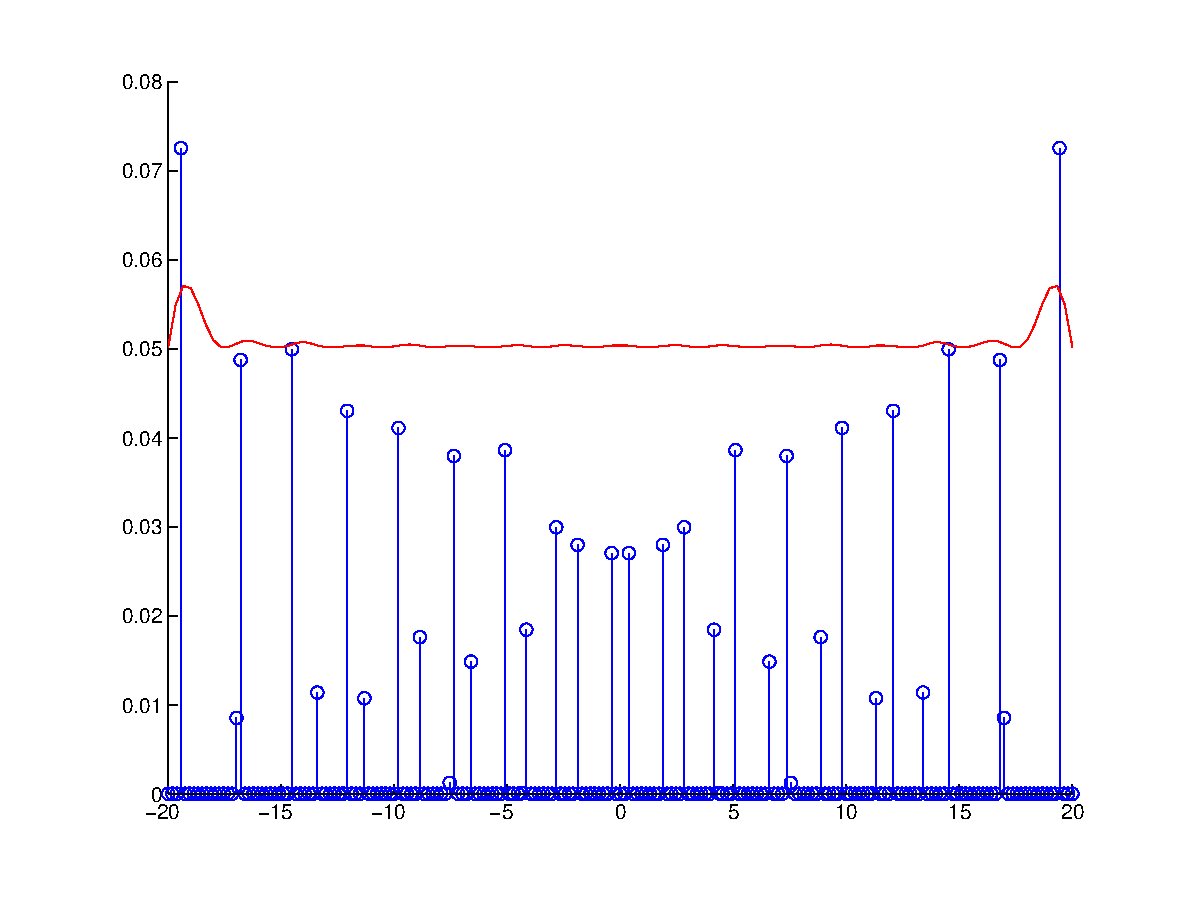
\includegraphics[scale=0.2]{support_b20}};
\node[int] at (4.1,0)  {\includegraphics[scale=0.2]{support_b10}};
\node[int] at (0,3.2)  {\includegraphics[scale=0.2]{support_b5}};
\node[int] at (4.1,3.2)  {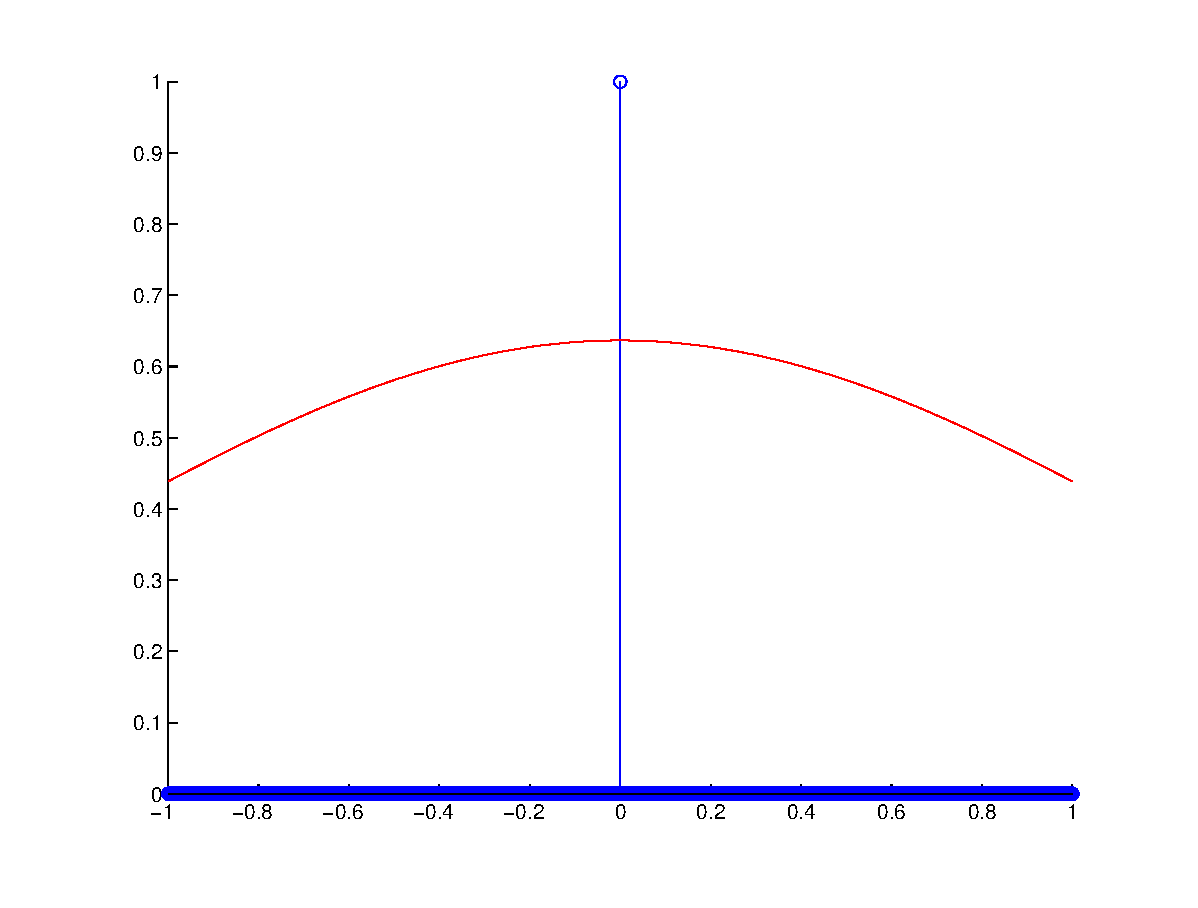
\includegraphics[scale=0.2]{support_b1}};
\end{tikzpicture}
\caption{\label{fig:cvx}
Support of the optimal density $\lambda$ that minimizes the asymptotic ML risk for the worst choice of $\theta \in [-\sigma b, \sigma b]$ (blue), for $b=1,5,10,20$ (clockwise). The red curve is the value of $K(\theta)$ under this density. 
}
\end{center}
\end{figure}


\begin{figure}
\begin{center}
\begin{tikzpicture}
\node at (0,0)  {\includegraphics[scale=0.25]{K_vs_b}};
\end{tikzpicture}
\caption{\label{fig:cvx2}
Asymptotic risk of the ML estimator under an optimal choice of the threshold density $\lambda$ versus the support of the parameter space $\Theta$.
}
\end{center}
\end{figure}

\begin{figure}
\begin{center}
\begin{tikzpicture}
\node[int] at (0,0)  {\includegraphics[scale=0.2]{opt_density_sig025}};
\node[int] at (4,0)  {\includegraphics[scale=0.2]{opt_density_sig1}};
\node[int] at (8,0)  {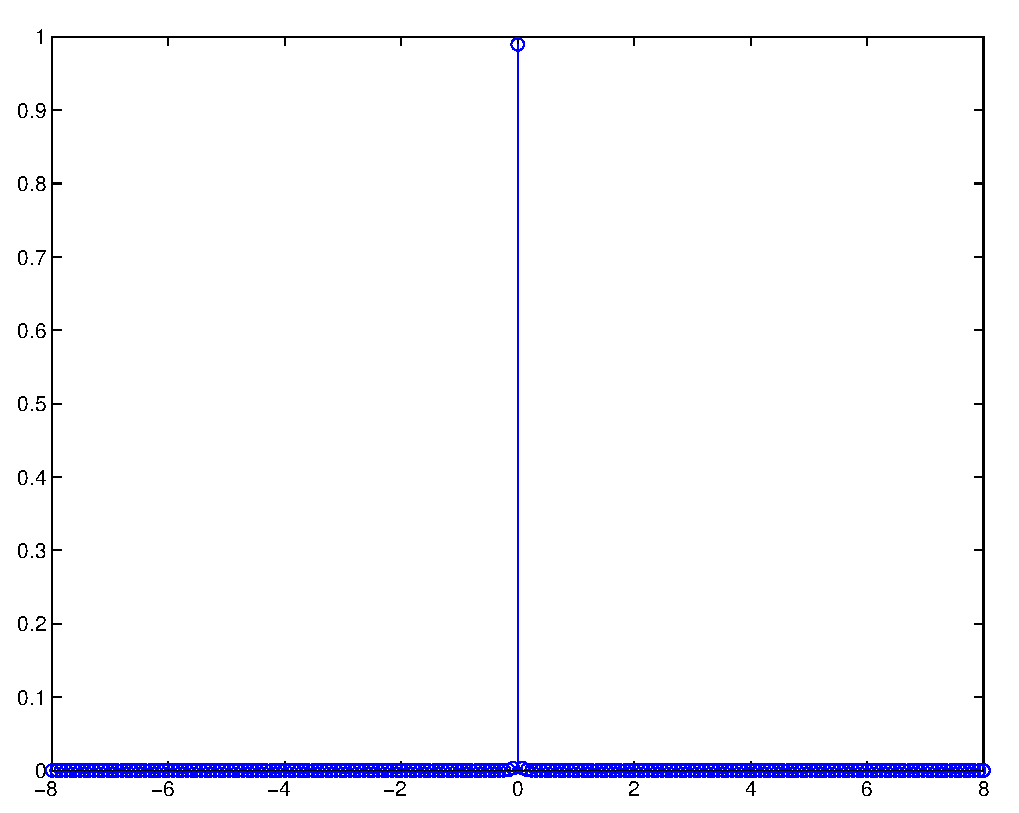
\includegraphics[scale=0.2]{opt_density_sig2}};
\end{tikzpicture}
\caption{\label{fig:opt_density}
The optimal asymptotic threshold density $\lambda$ that minimizes the expected asymptotic ML risk \eqref{eq:cvx_average} for a Gaussian prior for
 $\sigma/\sigma_\theta=0.25,1,2$ (left to right), where $\sigma_\theta^2$ is the variance of the prior. 
}
\end{center}
\end{figure}

\subsection{Average Asymptotic Risk}
Consider problem of minimizing the expected asymptotic risk $\mathbb E[ \sigma^2/K(\theta)]$ over all probability measures $\lambda(dt)$. This optimization problem can be written as follows:
\begin{align}
\label{eq:cvx_average}
\mathrm{minimize} \quad &  \sigma^2 \int \frac{\pi(d\theta)}{K(\theta)} =  \sigma^2 \int \frac{\pi(d\theta)}{ \int \eta \left( \frac{t-\theta}{\sigma}\right) \lambda(dt)}. \\ \nonumber
\mathrm{subject~to} \quad & \lambda(dt)\geq 0,\quad \int \lambda(dt) =1. 
\end{align}
Since the function $x \rightarrow 1/x$ is convex for positive values, \eqref{eq:cvx_average} defines a convex optimization problem in $\lambda$ whose solution depends on the the prior $\pi(\theta)$. The optimal asymptotic threshold density obtained as the solution to \eqref{eq:cvx_average} for a normal prior is illustrated in Fig.~\ref{fig:opt_density}, whereas Fig.~\ref{fig:dist_bound_Gaussian} illustrates the corresponding expected risk. The expected asymptotic risk for the uniform distribution is illustrated in Fig.~\ref{fig:dist_bound_uniform}. 
\par
%
\begin{figure}
\begin{center}
\begin{tikzpicture}
\node at (0,0) {\includegraphics[scale=0.5]{dist_bound_Gauss_prior}};
\node at (0,-2.5) {$\sigma/\sigma_\theta$};
\node[rotate = 90] at (-3.5,0) {(expected asymptotic risk)$/\sigma^2$};
\node at (1,0) {$\pi(\theta) = \mathcal N(0,\sigma_\theta^2)$ };
%\node at (-2,-1.05) {$\frac{\pi}{2}$};
%\node[rotate = -45] at (-1.8,1.2) {\color{red} true };
%\node[rotate = -70] at (-0.5,0) {\color{blue} bound };
\end{tikzpicture}
\caption{Expected asymptotic risk $\mathbb E (1/K(\theta))$ in estimation from threshold detectors versus $\sigma/\sigma_\theta$ for a Gaussian prior with variance $\sigma_\theta^2$. The optimal asymptotic threshold density $\lambda$ (red) is obtained by solving \eqref{eq:cvx_average}. The bound (blue) is obtained using \eqref{eq:upper_bound}.
\label{fig:dist_bound_Gaussian}  }
\end{center}
\end{figure}
%
\begin{figure}
\begin{center}
\begin{tikzpicture}
\node at (0,0) {\includegraphics[scale=0.5]{dist_bound_uniform_prior}};
\node at (0,-2.5) {$\sigma/\sigma_\theta$};
\node[rotate = 90] at (-3.5,0) {(expected asymptotic risk)$/\sigma^2$};
\node at (1,0) {$\pi(\theta)$ = Unif$(- \sqrt{3}\sigma_\theta, \sqrt{3}\sigma_\theta)$ };
%\node at (-2,-1.05) {$\frac{\pi}{2}$};
%\node[rotate = -45] at (-1.8,1.2) {\color{red} true };
%\node[rotate = -70] at (-0.5,0) {\color{blue} bound };
\end{tikzpicture}
\caption{Expected asymptotic risk $\mathbb E (1/K(\theta))$ in estimation from threshold detectors versus $\sigma/\sigma_\theta$ for a uniform prior with variance $\sigma_\theta^2$. The optimal asymptotic threshold density $\lambda$ (red) is obtained by solving \eqref{eq:cvx_average}. The bound (blue) is obtained using \eqref{eq:upper_bound}. 
\label{fig:dist_bound_uniform}  }
\end{center}
\end{figure}

As can be seen from Fig.~\ref{fig:opt_density}, for a normal prior with a small variance compared to the variance of the samples $\sigma^2$, the optimal density $\lambda$ is a mass distribution. As it turns out from the following proposition, the choice of  $\lambda$ to be a mass distribution leads to a general upper bound on the expected asymptotic risk, and not only on the minimal value of \eqref{eq:cvx_average}. 
\begin{prop}\label{prop:upper_bound}
Let $\theta_0 = \mathbb E \theta$. Then
\begin{equation}
\label{eq:upper_bound}
\mathbb E \frac{\sigma^2}{K(\theta)}  \leq \sigma^2 \int \frac{\pi(d\theta)}{\eta \left( \frac{\theta_0 - \theta}{\sigma} \right)}, 
\end{equation}
\end{prop}
\begin{proof}
Since the function $x \rightarrow 1/x$ is convex for positive values, Jensen's inequality applied to the RHS of \eqref{eq:cvx_average} leads to
\[
 \frac{\sigma^2}{K(\theta)} \leq \sigma^2 \int  \frac{ \lambda(dt)}{ \eta \left( \frac{t-\theta}{\sigma} \right)  }. 
\]
Therefore, the expected value of $\sigma^2/K(\theta)$ satisfies
\begin{align}
\mathbb E  \frac{\sigma^2}{K(\theta)}  \leq \sigma^2  \int \int \frac{\pi(d\theta) \lambda(dt) }{\eta \left( \frac{t - \theta}{\sigma} \right)}. \label{eq:upper_bound_proof}
\end{align}
The bound \eqref{eq:upper_bound} follows by using $\lambda = \delta_{\theta_0}$. 
\end{proof}
We note that since the function $1/\eta(x)$ is quasi-convex and symmetric, taking $\lambda = \lambda_{\theta_0}$ minimizes the RHS of \eqref{eq:upper_bound_proof} and leading to the tightest bound among the family bounds obtained after using Jensen's inequality.  \par
The bound \eqref{eq:upper_bound} is not trivial as long as the tail of the prior $\pi(\theta)$ is small enough such that the integral in the RHS of \eqref{eq:upper_bound} is finite. In general, this bound is tight whenever the support of the optimal distribution is a mass distribution at the origin. The following proposition implies that this bound is always tight as $\sigma / \sigma_\theta$ goes to infinity.
\begin{prop} \label{prop:asymp}
 For any prior $\pi(\theta)$ for which
\[
\int \frac{\pi(d\theta)}{\eta \left(\theta \right)} < \infty,
\]
we have 
\begin{align}
\label{eq:asymp}
\mathbb E [1/K(\theta)] = \frac{\pi}{2} + \left( \frac{\pi}{2} - 1\right) \left(\frac{\sigma_\theta}{\sigma} \right)^2 + o \left(\frac{1}{\sigma} \right)^3. 
\end{align}
as $\sigma_\theta / \sigma \rightarrow 0$. 
\end{prop}
\begin{proof}
It is enough to prove that  \eqref{eq:asymp} holds for the upper bound \eqref{eq:upper_bound}. First note that the condition in the proposition implies that all the moments of $\pi(\theta)$ exists, and in particular its second and third. The results follows by expanding the function $1/\eta(x)$ in a power series around zero as
\[
1/\eta(x) = \frac{\pi}{2} + \left(\frac{\pi}{2}-1 \right) x^2 + o(x^3).
\]
\end{proof}


\subsection{Discussion}
It follows from Prop.~\ref{prop:asymp} that the asymptotic expected risk converges to $\pi/2$ when the ratio between the variance of the distribution of $X_i$ to the variance of the prior tends to infinity. Therefore, we conclude that the minimal risk in the adaptive setting can be attained even in the distributed setting, as long as this ratio is large enough. Prop.~\ref{prop:asymp} also bounds the convergence rate of the expected risk to its optimal value, where we note that higher order terms in \eqref{eq:asymp} can be obtained by considering a higher order power series expansion of $1/\eta(x)$. \par
When the ratio $\sigma^2/ \sigma_\theta^2$ is large, the bound \eqref{eq:upper_bound} is tight and the probability measure $\lambda$ that minimizes the expected risk converges to a mass distribution at the expected value of $\theta$ according to its prior $\pi(\theta)$. Namely, all the encoders in this case report "$1$" whenever $X_i$ is larger than this expected value and ''$-1$'' otherwise. Intuitively, an accurate estimation of $\theta$ in this case is possible only if a sufficient mix of ''$1$''s and ''$-1$''s is obtained from the sample. When $\sigma_\theta^2$ is high, so is the probability of having a realization of $\theta$ away from its mean $\theta_0$. In this case, a threshold detector located at $\theta_0$ may have a strong bias toward one of ''$1$'' or ''$-1$'', unless the variance of the samples $\sigma^2$ is also relatively large. Indeed, as illustrated in Figs~\ref{fig:opt_density} and \ref{fig:dist_bound_Gaussian}, when $\sigma^2$ is small compared to $\sigma_\theta^2$, the bound in Prop.~\ref{prop:upper_bound} is not tight and the optimal asymptotic threshold density $\lambda$ is supported by multiple points. As illustrated in Figs~\ref{fig:dist_bound_Gaussian} and Figs~\ref{fig:dist_bound_uniform}, when the ratio $\sigma/\sigma_\theta$ is small the expected asymptotic risk, and therefore the relative efficiency of any asymptotic local minimax optimal estimator, is higher than $\pi/2$ and cannot be uniformly bounded in this ratio regardless of the threshold distribution $\lambda$. For example, if the prior information on $\theta$ indicates that it lays in the interval $[-1,1]$ with a uniform probability and the variance of the observations is $\sigma^2 = 0.02$, then the asymptotic expected relative efficiency is $~\approx 8.25$. This number goes down to $~\approx 3.02$ for $\sigma^2 = 0.2$. 
\\

To summarize, we conclude that when the prior information on $\theta$ provides a reasonable localization of its value compared to the variance of the measurements, then the relative efficiency \eqref{eq:relative_efficiency} of the ML estimator is $\pi/2$. On the other hand, the relative efficiency of any local asymptotic minimax estimator can be very high if the variance of the measurements is very small compared to the apriori uncertainty in $\theta$, even under the optimal threshold distribution $\lambda$. 

%For example, when $\pi(\theta)$ is a zero mean normal with variance $\sigma_\theta^2$ and $\sigma / \sigma_\theta=1$, the upper bound in \eqref{eq:upper_bound} equals $3.563$. With $\sigma/\sigma_\theta=2$ it equals $1.748$. The behavior of this bound is illustrated in Fig.~\ref{fig:dist_bound_Gaussian}. For large $\sigma/\sigma_\theta$ it converges to $\sigma^2 \pi/2$. For small $\sigma$ the expression above can be very large, but, as explained below, in this case the bound is not tight. 

\section{Conclusions \label{sec:conclusions}}
We considered the relative efficiency in estimating the mean of a normal distribution from a single-bit encoding of each sample from this distribution. For the adaptive setting, we have shown that this minimal relative efficiency is $\pi/2$, namely there is a penalty factor of at least $\pi/2$ on the asymptotic mean square error risk in estimating the mean compared to an estimator that has full access to the sample. We also showed that this lower bound is tight by presenting an adaptive estimation procedure that attains it.
%but ignores the prior distribution on the parameter space.
In addition, we characterized the single-bit message that minimizes the next step MSE, and described an estimation procedure that is based on a sequence of one-step optimal messages. We leave open the questions whether this estimator attains the minimal efficiency and whether it leads to an estimation scheme which is globally optimal in the adaptive setting. \par
For the distributed setting, we considered the estimation from threshold detection under the assumption that density of the threshold values converges to a probability distribution. For this setting, we characterized the risk attained by the maximum likelihood estimator, and showed that this estimator is local asymptotic minimax. In addition, we showed that when the variance of the underlying normal distribution is high compared to the size of the variance of the prior on the unknown mean, the asymptotic relative efficiency in this setting converges to $\pi/2$. Namely, under this conditions, there is no loss in efficiency compared to the adaptive case. Nevertheless, this relative efficiency can be very high whenever the variance of the underlying distribution is very small compared to the apriori uncertainty in $\theta$. We leave open the question whether there exists a distributed one-bit estimation scheme that achieves relative efficiency close to $\pi/2$ even when the apriori uncertainty in $\theta$ is high compared to the variance of the underlying normal distribution.

%\section*{ACKNOWLEDGMENT}
%This research is supported in parts by...
%Tsachy Weissman, Stefano Rini, Robert Gray.

\appendix

\section{Proofs}
In this appendix we provide detailed proofs of our main results as described in Section~\ref{sec:sequential}.

\subsection*{Proof of Theorem~\ref{thm:adpative_lower_bound}}

We first prove the following two lemmas:
\begin{lem} \label{lem:bound_intervals}
For any $x_1 \geq \ldots \geq x_n \in \mathbb R$, we have 
\begin{equation}
\frac{ \left(  \sum_{k=1}^n (-1)^{k+1}\phi(x_k) \right)^2} 
{\left( \sum_{k=1}^n (-1)^{k+1} \Phi(x_k) \right)\left(1- \sum_{k=1}^n (-1)^{k+1} \Phi(x_k) \right)  } \leq \frac{2} {\pi}. \label{eq:bound_intervals}
\end{equation}
\end{lem}
\begin{lem} \label{lem:fisher_bound}
Let $X\sim \mathcal N(\theta,\sigma^2)$ and assume that 
\[
M(X) = \begin{cases} 1,& X \in A, \\
-1, & X \notin A.
\end{cases}
\]
Then the Fisher information of $M$ with respect to $\theta$ is bounded from above by $2/(\pi \sigma^2)$.
\end{lem}

\subsubsection*{Proof of Lemma~\ref{lem:bound_intervals}}
We use induction on $n \in \mathbb N$. For the base case $n=1$ we have 
\begin{equation} \label{eq:induction_base}
\eta(x) \triangleq \frac{  \phi^2(x)} 
{\Phi(x) \left(1 - \Phi(x) \right) }. 
\end{equation}
Taking the logarithm of \eqref{eq:induction_base} and differentiating, we conclude that any point $x$ that maximizes \eqref{eq:induction_base} satisfies
\[
x = \phi(x) \left( \Phi(x) -\frac{1}{2} \right).
\]
However, since $x > \phi(x) \left( \Phi(x) -\frac{1}{2} \right)$ for all $x > 0$, the only point that satisfies the last condition is $x=0$. At this point \eqref{eq:induction_base} equals $2/\pi$. \par
Assume now that \eqref{eq:bound_intervals} holds for all integers up to some $n = N-1$ and consider the case $n = N$. The maximal value of \eqref{eq:bound_intervals} is attained for the same $(x_1,\ldots,x_N) \in \mathbb R^N$ that attains the maximal value of 
\begin{align*}
& g(x_1,\ldots, x_N) \triangleq 2 \log \left(  \sum_{k=1}^{N} (-1)^{k+1} \phi(x_k) \right) - \log
\left( \sum_{k=1}^N (-1)^{k+1} \Phi(x_k) \right)
-\log \left(1 -  \sum_{k=1}^N (-1)^{k+1} \Phi(x_k) \right) \\
& = 2 \log \delta_N - \log \Delta_N - \log \left(1 - \Delta_N  \right),
\end{align*}
where we denoted $\delta_N \triangleq \sum_{k=1}^{N} (-1)^{k+1} \phi(x_k)$ and $\Delta_N =  \sum_{k=1}^N (-1)^{k+1} \Phi(x_k)$. The derivative of $g(x_1,\ldots,x_N)$ with respect to $x_k$ is given by
\[
\frac{\partial  g}{\partial x_k} = \frac{2 (-1)^{k+1} \phi'(x_k)}{\delta_N} -\frac{(-1)^{k+1} \phi(x_k)}{\Delta_N } + \frac{(-1)^{k+1} \phi(x_k)}{1-\Delta_N }.
\]
Using the fact that $\phi'(x) = -x \phi(x)$, we conclude that the gradient of $g$ vanishes only if
\[
x_k = \frac{\delta_N}{2} \left( \frac{1}{\Delta_N} - \frac{1}{1-\Delta_N} \right),\quad k=1,\ldots,N.
\]
In particular, the condition above implies $x_1 = \ldots = x_N$. If $N$ is odd then for $x_1=\ldots =x_N$ we have that \eqref{eq:bound_intervals} equals $\eta(x_1)$, which was previously shown to be smaller than $\pi/2$. If $N$ is even, then for any constant $c$ the limit of \eqref{eq:bound_intervals} exits as $(x_1,\ldots,x_N)\rightarrow (c,\ldots,c)$ and equals zero. Therefore, the maximum of \eqref{eq:bound_intervals} is not attained at this line. We now consider the possibility that \eqref{eq:bound_intervals} is maximized at the borders, as one or more of the coordinates of $(x_1,\ldots,x_N)$ approaches plus or minus infinity. For simplicity we only consider the cases where $x_N$ goes to minus infinity or $x_1$ goes to plus infinity (the general case where the first $m$ coordinates goes to infinity or the last $m$ to minus infinity is obtained using similar arguments). Assume first $x_N \rightarrow -\infty$. Then  \eqref{eq:bound_intervals} equals
\begin{align*}
\frac{ \left(  \sum_{k=1}^{N-1} (-1)^{k+1}\phi(x_k) \right)^2} 
{\left( \sum_{k=1}^{N-1} (-1)^{k+1} \Phi(x_k) \right)\left(1- \sum_{k=1}^{N-1} (-1)^{k+1} \Phi(x_k)  \right) } ,
\end{align*}
which is smaller than $2/\pi$ by the induction hypothesis. Assume now that $x_1 \rightarrow \infty$. Then 
\eqref{eq:bound_intervals} equals
\begin{align*}
& \frac{ \left(  \sum_{k=2}^{N} (-1)^{k+1}\phi(x_k) \right)^2} 
{\left( 1 + \sum_{k=2}^{N} (-1)^{k+1} \Phi(x_k) \right)\left(1- 1 - \sum_{k=2}^{N} (-1)^{k+1} \Phi(x_k)  \right) }  \\
& = \frac{ \left(  -\sum_{m=1}^{N} (-1)^{m+1}\phi(x'_m) \right)^2} 
{\left( 1 - \sum_{m=1}^{N-1} (-1)^{m+1} \Phi(x'_{m}) \right)\left( \sum_{m=1}^{N-1} (-1)^{m+1} \Phi(x'_{m})  \right) },
\end{align*}
where $x'_{m} = x_{m+1}$. The last expression is also smaller than $2/\pi$ by the induction hypothesis. This proves Lemma~\ref{lem:bound_intervals}. \\

\subsubsection*{Proof of Lemma~\ref{lem:fisher_bound}}
The Fisher information of $M$ with respect to $\theta$ is given by
\begin{align}
I_\theta & =  \mathbb E \left[ \left( \frac{d}{d\theta} \log P\left( M | \theta \right) \right)^2 |\theta \right] \nonumber \\
& = \frac{ \left(\frac{d}{d\theta} P(M=1|\theta) \right)^2}{P(M=1| \theta)} + \frac{ \left(\frac{d}{d\theta} P(M=-1|\theta) \right)^2} {P(M=-1| \theta)} \nonumber \\
& \overset{(a)}{=} \frac{ \left( - \int_A \phi' \left( \frac{x-\theta}{\sigma} \right)dx \right)^2} {\sigma^2 P(M=1| \theta) } + \frac{ \left( \int_A \phi' \left( \frac{x-\theta}{\sigma} \right)dx \right)^2} { \sigma^2P(M=-1| \theta) } \nonumber \\ 
& = \frac{\left( \int_A \phi'\left( \frac{x-\theta}{\sigma} \right) dx \right)^2 }{  \sigma^2 P(M=1 | \theta) \left(1-P(M=1|\theta) \right)  }, \nonumber \\
& = \frac{\left( \int_A \phi'\left( \frac{x-\theta}{\sigma} \right) dx \right) \left( \int_A \phi'\left( \frac{x-\theta}{\sigma} \right) dx \right)}{  \sigma^2 \left( \int_A \phi \left( \frac{x-\theta}{\sigma} \right) dx \right)  \left(1- \int_A \phi \left( \frac{x-\theta}{\sigma} \right) dx \right) }, \label{eq:lem_fisher_bound_proof1}
\end{align}
where differentiation under the integral sign in $(a)$ is possible since $\phi(x)$ is differentiable with absolutely integrable derivative $\phi'(x) = -x\phi(x)$. Regularity of the Lebesgue measure implies that for any $\epsilon>0$, there exists a finite number $k$ of disjoint open intervals $I_1,\ldots I_k$ such that 
\[
\int_{A\setminus \cup_{j=1}^k I_j }  dx < \epsilon \sigma^2,
\]
which implies that for any $\epsilon' > 0$, the set $A$ in \eqref{eq:lem_fisher_bound_proof1} can be replaced by a finite union of disjoint intervals without increasing $I_\theta$ by more than $\epsilon'$. It is therefore enough to proceed in the proof assuming that $A$ is of the form
\[
A = \cup_{j=1}^k (a_j,b_j),
\]
with $\infty \leq a_1 \leq \ldots a_k$, $b_1 \leq b_k \leq \infty$ and $a_j \leq b_j$ for $j=1,\ldots,k$. Under this assumption we have
\begin{align*}
\mathbb P(M_n=1) & = \sum_{j=1}^k \mathbb P\left(X_n \in (a_j,b_j) \right)  \\
& = \sum_{j=1}^k \left( \Phi \left(\frac{b_j-\theta}{\sigma} \right) -  \Phi \left(\frac{a_j-\theta}{\sigma} \right)  \right),
\end{align*}
so \eqref{eq:lem_fisher_bound_proof1} can be rewritten as
\begin{align}
& =   \frac { \left( \sum_{j=1}^{k} \phi \left(\frac{a_j-\theta}{\sigma} \right) - \phi \left( \frac{b_j-\theta} {\sigma} \right)  \right)^2 } 
{\sigma^2 \left( \sum_{j=1}^k \Phi \left( \frac{b_j-\theta }{\sigma}\right) - \Phi \left( \frac{a_j-\theta }{\sigma}\right)  \right) }  \nonumber \\
& \times \frac {1} 
{1- \left( \sum_{j=1}^k \Phi \left( \frac{b_j-\theta }{\sigma}\right) - \Phi \left( \frac{a_j-\theta }{\sigma}\right)  \right) } 
\label{eq:lemma_J}
\end{align}
The proof of Lemma~\ref{lem:fisher_bound} is completed since it follows from~\ref{lem:bound_intervals} that for any $\theta \in \mathbb R$ and any choice of the intervals endpoints, \eqref{eq:lemma_J} is smaller than $2/(\sigma^2 \pi)$. \\


We now consider the proof of Thm.~\ref{thm:adpative_lower_bound}. In order to bound from above the Fisher information of any set of $n$ single-bit messages with respect to $\theta$, we first note that without loss of generality, each message $M_i$ can be written in the form
\begin{equation}
\label{eq:general_messages}
M_i = \begin{cases}
X_i \in A_i & 1, \\
X_i \notin A_i & -1,
\end{cases} 
\end{equation}
where $A_i \subset \mathbb R$ is a Lebesgue measurable set. Indeed, any measurable function $M(X_i) \in \{-1,1\}$ can be written in the form \eqref{eq:general_messages} with $A_i = M^{-1}(1)$. Consider the conditional distribution $P({M^n|\theta})$ of $M^n$ given $\theta$. We have 
\begin{align}
P\left( M^n | \theta \right) & =  \prod_{i=1}^n P\left(M_i | \theta, M^{i-1} \right), \label{eq:adpt_lower_bound_proof:1}
\end{align}
where $P\left(M_i =1 | \theta, M^{i-1}  \right) = \mathbb P\left( X_i \in A_i\right)$. Going back to \eqref{eq:adpt_lower_bound_proof:1}, it follows that the Fisher information of $M^n$ with respect to $\theta$ is given by 
\begin{align}
I_\theta(M^n) = \sum_{i=1}^n I_\theta (M_i|M^{i-1}),
\label{eq:fisher_information}
\end{align}
where $I_\theta (M_i|M^{i-1})$ is the Fisher information of the distribution of $M_i$ given $M^{i-1}$. From Lemma~\ref{lem:fisher_bound} it follows that $I_\theta (M_i|M^{i-1}) \leq 2/(\pi \sigma^2)$. The Van Trees inequality \cite{van2004detection, gill1995applications} now implies 
\begin{align*}
\mathbb E \left( \theta_n - \theta \right)^2 &  \geq \frac{1}{ \mathbb E I_\theta(M^n) + I_0} \\
& = \frac{1}{ \sum_{i=1}^n I_\theta (M_i | M^{i-1} ) + I_0} \\
& \geq \frac{1}{ 2n/(\pi \sigma^2) + I_0}.
\end{align*}

\QEDA

\subsection*{Proof of Theorem~\ref{thm:sgd}}
The algorithm given in \eqref{eq:sgd_alg} and \eqref{eq:sgd_est} is a special case of a more general class of estimation procedures given in \cite{polyak1992acceleration}. In particular, Theorem~\ref{thm:sgd} is follows directly from the following simplified version of \cite[Thm. 4]{polyak1992acceleration}:
\begin{thm}{\cite[Thm. 4]{polyak1992acceleration}} \label{thm:polyak_juditsky}
Let 
\[
X_i = \theta + Z_i,\quad i=1,\ldots,n.
\]
Define 
\begin{align*}
\theta_i & = \theta_{i-1} + \gamma_i \varphi(X_i - \theta_{i-1}), \\
\widehat{\theta}_n & = \frac{1}{n} \sum_{i=0}^{n-1} \theta_i,
\end{align*}
where the $Z_i$s are $\mathcal N(0,\sigma^2)$ and independent of each other, the sequence $\left\{ \gamma_i \right\}_{i=1}^\infty$ satisfies conditions (i) and (ii) in Theorem~\ref{thm:sgd}, and $\left| \varphi(x) \right| \leq K_1(1+x)$ for some $K_1$. Define $\psi(x) = \mathbb E \varphi(x+Z_1)$, $\chi(x) = \mathbb E \varphi^2(x+Z_1)$ and assume that $\psi(0)=0$, $x\psi(x) >0$ for all $x\neq 0$, $\chi(x)$ is continuous at zero, and that $\psi(x)$ is differentiable at zero with $\psi'(0)>0$. Moreover, assume that there exists $K_2$ and $0<\lambda \leq 1$ such that
\[
\left| \psi(x) - \psi'(0)x \right|\leq K_2 |x|^{1+\gamma}.
\]
Then $\widehat{\theta}_n \rightarrow \theta$ almost surely and $ \sqrt{n}(\widehat{\theta}_n - \theta)$ converges in distribution to $\mathcal N(0,V)$, where
\[
V = \frac{ \chi(0)} {\psi'^2(0)}. 
\]
\end{thm}


Using the notation in Theorem~\ref{thm:polyak_juditsky}, we set $\varphi(x) = \sgn(x)$ and $Z_i = X_i - \theta$. We have: 
\[
\chi(x) = \mathbb E \varphi^2(x+Z_1),
\]
so $\chi(0) = 1$. In addition,
\begin{align*}
\psi(x) & = \mathbb E \sgn(x+ Z_1) = \int_{-\infty}^\infty \sgn(x+z) \frac{1}{\sqrt{2\pi}\sigma} e^{-\frac{z^2}{\sigma^2}} dz \\
& = \int_{-x}^\infty \frac{1}{\sqrt{2\pi}\sigma} e^{-\frac{z^2}{\sigma^2}} dz -\int_{-\infty}^{-x} \frac{1}{\sqrt{2\pi}\sigma} e^{-\frac{z^2}{\sigma^2}} dz.
\end{align*}
This leads to 
\begin{align*}
\psi'(x) & = \frac{1}{\sqrt{2\pi}\sigma} e^{-\frac{x^2}{\sigma^2}} dz +\frac{1}{\sqrt{2\pi}\sigma} e^{-\frac{z^2}{\sigma^2}} dz,
\end{align*}
so $\psi'(0) = \frac{2}{\sqrt{2\pi}\sigma}$. It is now easy to verify that the rest of the conditions in Theorem~\ref{thm:polyak_juditsky} are fulfilled for any $\lambda > 0$. Since 
\[
\frac{\chi(0)}{\psi'^2(0)} = \frac{\pi \sigma^2}{2},
\]
Theorem~\ref{thm:sgd} follows from Theorem~\ref{thm:polyak_juditsky}. \QEDA


\subsection*{Proof of Theorem~\ref{thm:opt_one_step}}
In this subsection we prove lemmas \ref{lem:adaptive} and \ref{lem:unique} which lead to Theorem~\ref{thm:opt_one_step}. 

\subsubsection*{Proof of Lemma \ref{lem:adaptive}}
Since any single-bit message $M(u) \in \{0,1\}$ is characterized by two decision region $A_1 = M^{-1}(1)$ and $A_{-1} = M^{-1}(-1)$, it follows that $\mathbb E \left[ U | M(U) \right]$ assumes only two values: $\mu_1 = \mathbb E \left[ U | M(U) = 1 \right]$ and $\mu_{-1} = \mathbb E \left[ U | M(U) = -1 \right]$. We claim that a necessary condition for $M(u)$ to be optimal is that the sets $A_1$ and $A_{-1}$ are, modulo a set of measure $P(du)$ zero, the Voronoi sets on $\mathbb R$ corresponding to the points $\mu_1$ and $\mu_{-1}$, respectively. Indeed, assume by contradiction that for such an optimal partition there exists a set $B \subset A_{1}$ with $\mathbb P (U \in B) >0$ such that $\left( b-\mu_{1} \right)^2 > \left( b- \mu_{-1} \right)^2$. The expected square error in this partition satisfies:
\begin{align*}
& \int_{\mathbb R} \left( u - \mathbb E[U|M(u)]  \right)^2 P(du) = \int_{A_1} (u- \mu_1)^2 P(du) + \int_{A_{-1}} (u- \mu_{-1})^2 P(du) \\
& = \int_{A_1\setminus B} (u- \mu_1)^2 P(du) +  \int_{B} (u- \mu_1)^2 P(du) + \int_{A_{-1}} (u- \mu_{-1})^2 P(du) \\
& > \int_{A_1\setminus B} (u- \mu_1)^2 P(du) +  \int_{B} (u- \mu_2)^2 P(du) + \int_{A_{-1}} (u- \mu_{-1})^2 P(du),
\end{align*}
so clearly, the partition $A_1' = A_1 \setminus B$, $A_{-1}' = A_{-1} \cup B$ attains lower error variance which contradicts the optimality assumption and proves our claim. It is evident that Voronoi partition of the real line corresponding to $\mu_1$ and $\mu_{-1}$ is of the form $A_{-1} = (-\infty,\tau)$, $A_{1} = (\tau, \infty)$ where the point $\tau$ is of equal distance from $\mu_1$ and $\mu_{-1}$, namely $\tau = \frac{\mu_1 + \mu_{-1}}{2}$. From these two conditions (which are a special case of the conditions derived in \cite{1056489} for two quantization regions) we conclude that $\tau$ must satisfy the equation
\[
2 \tau = \frac{\int_{\tau}^\infty u P(du)}{\int_{\tau}^\infty P(du)} + \frac{\int_{-\infty}^{\tau} u P(du)}{\int_{-\infty}^{\tau} P(du)}.
\] 
\QEDA

\subsubsection*{Proof of Lemma \ref{lem:unique}} 
Any solution to \eqref{eq:lem_fixed_point} is a solution to $h^+(x) = h^-(x)$ where
\[
h^+(x) = \frac{\int_x^\infty uf(u)du}{\int_x^\infty f(u)du} - x 
\]
and
\[
h^-(x) = x - \frac{\int_{-\infty}^x uf(u)du}{\int_{-\infty}^x f(u)du}.
\]
We now prove that $h^+(x)$ is monotonically decreasing while $h^-(x)$ is increasing, so they meet at most at one point. The derivative of $h^-(x)$ is given by
\begin{equation} 
\label{eq:one_step_proof_derivative}
1 - \frac{ f(\tau) \int_{-\infty}^\tau f(x) (\tau-x)dx } {\left( \int_{-\infty}^\tau f(x) dx \right)^2}.
\end{equation}
Denote $F(x) = \int_{-\infty}^x f(u)du$. Using integration by parts in the numerator and from the fact that $\lim_{\tau \rightarrow -\infty}  \tau \int_{-\infty}^\tau f(x) dx = 0$, the last expression can be written as
\[
1- \frac{ f(\tau) \int_{-\infty}^\tau F(x) dx}
 {\left( F(\tau) \right)^2}.
\]
Log-concavity of $f(x)$ implies log-concavity of $F(x)$, so that we can write $F(x) = e^{g(x)}$ for some concave and differentiable function $g(x)$. Moreover, we have $f(x) = g'(x)e^{g(x)}$ where, by concavity of $g(x)$, the derivative $g'(x)$ of $g(x)$ is non-increasing. With these notation we have
\begin{align*}
\frac{ f(\tau) \int_{-\infty}^\tau F(x) dx}
 {\left( F(\tau) \right)^2} & = \frac{g'(\tau)e^{g(\tau)} \int_{-\infty}^\tau e^{g(x)}dx }{ e^{2g(\tau)} } \\
 & = e^{-g(\tau)} \int_{-\infty}^\tau g'(\tau) e^{g(x)} dx  \\
 & \leq e^{-g(\tau)} \int_{-\infty}^\tau g'(x) e^{g(x)} dx \\
 & = e^{-g(\tau)} F(\tau) = 1.
\end{align*}
(where the second from the last step follows since $g'(x) \leq g'(\tau)$ for any $x\leq \tau$). If follows that \eqref{eq:one_step_proof_derivative} is non-negative and thus $h^-(x)$ is monotonically increasing. Since
\[
h^+(-x) = x - \frac{ \int_{-\infty}^{x} uf(-u)du}{ \int_{-\infty}^x f(-u) du }, 
\]
the fact that $h^+(x)$ is monotonically decreasing follows from similar arguments. Moreover, since the derivatives of $h^+(x)$ and $h^-(x)$ never vanish at the same time over any open interval, their difference cannot be constant over any interval. Finally, since 
\begin{align*}
 \lim_{x\rightarrow -\infty} h^+(x) =  \lim_{x\rightarrow \infty} h^-(x)
\end{align*}
and since non of these functions are constant, monotonicity of $h^+(x)$ and $h^-(x)$ implies that they must meet at some $x\in \mathbb R$. \QEDA


\subsection*{Proof of Theorem~\ref{thm:LAN}}
We will prove that the distribution of $M^n$ defines a local asymptotic normal (LAN) family of probability distributions with \emph{precision} parameter $K(\theta)/\sigma^2$. The statements in the theorem then follows from the local asymptotic minimax theorem of LAN families \cite{van2000asymptotic}. \\

The probability mass distribution of $M^n$ is given by
\[
P_\theta(m^n) =  \prod_{i=1}^n  \Phi \left( m_i \frac{t_i - \theta}{\sigma} \right). 
\]
Consider the log-likelihood ratio under a sequence of local alternatives $\theta' = \theta + h/\sqrt{n}$ for some $h\in \mathbb R$:
\begin{align}
\log \frac{ P_{\theta + \frac{h}{\sqrt{n}}}(M^n)} { P_\theta (M^n) }& =  \sum_{i=1}^n \log \left(  \Phi \left( \frac{M_i}{\sigma} (t_i - \theta - h/\sqrt{n} ) \right)\right)  - \sum_{i=1}^n \log \left( \Phi \left( M_i \frac{t_i - \theta}{\sigma} \right) \right). \label{eq:LAN_proof1}
\end{align}
Using the Taylor expansion of $\log \Phi(x)$, \eqref{eq:LAN_proof1} can be written as
\[
- h \sum_{i=1}^n  \frac{M_i}{\sqrt{n} \sigma }  \frac{ \phi \left(M_i\frac{t_i-\theta}{\sigma} \right)} {\Phi \left( M_i \frac{t_i-\theta}{\sigma} \right) }  - \frac{h^2}{2 \sigma^2 n} \sum_{i=1}^n   \left( \frac{\phi' \left(M_i \frac{t_i-\theta}{\sigma} \right) }{\Phi\left(M_i \frac{t_i-\theta}{\sigma}\right) }- \frac{ \phi^2\left(M_i \frac{t_i-\theta}{\sigma} \right)}{\Phi^2\left(M_i \frac{t_i-\theta}{\sigma} \right)}   \right) + o(1)
\] 

The proof is completed by proving the following two lemmas:
\begin{lem} \label{lem:LAN1}
For $i=1,\ldots,n$ denote 
\[
U_i = -M_i \frac{ \phi \left( M_i \frac{t_i - \theta}{\sigma} \right)}{ \Phi \left( M_i \frac{t_i - \theta}{\sigma}\right) }. 
\]
Then 
\[
\frac{1}{\sqrt{n}} \sum_{i=1}^n U_i \overset{D}{\rightarrow} \mathcal N\left(0, K(\theta) \right). 
\]
\end{lem}
\begin{lem} \label{lem:LAN2}
For $i=1,\ldots,n$ denote
\[
V_i =  \left[ \frac{\phi' \left(M_i \frac{t_i-\theta}{\sigma} \right) }{\Phi\left(M_i \frac{t_i-\theta}{\sigma}\right) }- \frac{ \phi^2\left(M_i \frac{t_i-\theta}{\sigma} \right)}{\Phi^2\left(M_i \frac{t_i-\theta}{\sigma} \right)} \right] .
\]
Then 
\[
\frac{1}{n} \sum_{i=1}^n V_i \overset{a.s.}{\rightarrow} K(\theta). 
\]
\end{lem}

\subsubsection*{Proof of Lemma~\ref{lem:LAN1}} 
We have that $\mathbb E  U_i= 0$. In addition,
\[
\mathbb E U_i^2 = \frac{ \phi^2 \left( \frac{t_i-\theta}{\sigma} \right) } { \Phi \left( \frac{t_i-\theta}{\sigma} \right) \left(1- \Phi \left( \frac{t_i-\theta}{\sigma} \right) \right)},
\]
and therefore
\[
\frac{1}{n} \sum_{i=1}^n \mathbb E U_i^2 \rightarrow K(\theta).
\]

We now verify that the sequence $\{ U_i,\,i=1,2,\ldots \}$ satisfies Lyaponov's condition: for any $\delta>0$ we have that 
\[
\mathbb E \left| U_i \right|^{2+\delta} = \phi^{2+\delta} \left(\frac{t_i-\theta} {\sigma } \right)   \left( \frac{1}{\Phi^{2+\delta} \left(\frac{t_i-\theta}{\sigma }\right)} + \frac{1}{1-\Phi^{2+\delta} \left(\frac{t_i-\theta}{\sigma }\right)} \right),
\]
and
\begin{equation}
\frac{\sum_{i=1}^n \mathbb E \left| U_i \right|^{2+\delta} }{ \left( \sqrt{\sum_{i=1}^n \mathbb E U_i^2 } \right)^{2+\delta}} = 
\frac{ \frac{1}{n^{1+\delta}} \sum_{i=1}^n \mathbb E U_i^{2+\delta} }{ \left(\frac{1}{n} \sum_{i=1}^n \mathbb E U_i^2  \right) \left(\frac{1}{n} \sum_{i=1}^n \mathbb E U_i^2  \right)^\delta}. 
\label{eq:Lyaponov}
\end{equation}
As $n$ goes to infinity, we have
\[
\frac{1}{n}\sum_{i=1}^n \mathbb E \left| U_i \right|^{2+\delta}  \rightarrow  \int \phi^{2+\delta} \left(\frac{t-\theta}{\sigma }\right) \left( \frac{1}{\Phi^{2+\delta}\left(\frac{t-\theta}{\sigma }\right)} + \frac{1}{1-\Phi^{2+\delta} \left(\frac{t-\theta}{\sigma }\right)} \right) \lambda(dt),
\]
so the numerator in \eqref{eq:Lyaponov} goes to zero. Since the denumerator in \eqref{eq:Lyaponov} goes to $(K(\theta))^{1+\delta})$, the entire expression goes to zero and hence Lyaponov's condition is satisfied. From Lyaponov's central limit theorem we conclude that 
\[
\frac{1}{\sqrt{n}} \sum_{i=1}^n U_i \overset{D}{\rightarrow} \mathcal N\left(0,K(\theta) \right). 
\]
\QEDA

\subsubsection*{Proof of Lemma~\ref{lem:LAN2}} 

Since $\phi'(x) = -x \phi(x)$, we have that
\[
\mathbb E V_i =  \frac{\phi^2 \left(\frac{ t_i-\theta}{\sigma} \right) } { \Phi \left(\frac{ t_i-\theta}{\sigma} \right)  \left(1-\Phi \left(\frac{ t_i-\theta}{\sigma} \right)  \right)},
\]
and thus
\[
\frac{1}{n} \sum_{i=1}^n \mathbb E V_i =  \frac{1}{n} \sum_{i=1}^n  \frac{\phi^2\left( \frac{t_i-\theta}{\sigma} \right)} { \Phi \left( \frac{t_i - \theta}{\sigma} \right)\left(1-\Phi \left( \frac{t_i - \theta}{\sigma} \right) \right)} \rightarrow K(\theta).  
\]
It follows from Kolmogorov's law of large numbers (e.g. \cite[Thm. 10.2.3]{sen1994large}) that
\[
\frac{1}{n} \sum_{i=1}^n \mathbb E V_i \overset{a.s.}{\rightarrow} K(\theta). 
\]
\QEDA


%%%%%%%%%%%%%%%%%%%%%%%%%%%%%%%%%%%%%%%%%%%%%%%%%%%%%%%%%%%%%%%%%%%%%%%%%%%%%%%%
\bibliographystyle{IEEEtran}
\bibliography{IEEEabrv,/Users/Alon1/LaTex/bibtex/sampling}


\section{Related Results in Source Coding}
The estimation problem we consider can be seen as the quantization, compression or encoding of the samples, and the  decoding of the parameter $\theta$ from the encoded version of the sample. Therefore, this problem is closely related to various setting in coding and information theory. The goal of this section is to illustrates this connection and review related results that are relevant in our case. 

%As opposed to the aforementioned line of works, we focus on estimation of samples taken from a single distribution in the finite blocklength performance. We are interested in particular in addition restrictions on the communication and information sharing between the encoders. For example, our main focus is the case where the observer must communicate a single bit upon drawing from the distribution. This is in contrast to the asymptotic setting where the observer can encode the outcome of $n$ draws at once using a single $n$ bit message. Alternately, such setting can be seen as having $n$ different observers, each is capable of observing a single realization and transmit a single bit. 

%{\color{red} The Van Trees inequality was extended to the estimation of multiple parameters in \cite{bobrovsky1987}. It is closely related with the }


\subsection{Statistical Inference under Communication Constraints}
The works \cite{han1987hypothesis, zhang1988estimation, 720540} consider various problems of statistical inference under multiterminal lossy compression. In the setting of \cite{han1987hypothesis, zhang1988estimation, 720540}, each terminal $I$ observes $n$ samples from the distribution and is allotted $nR_i$ bits to communicate its estimate.% Consequently, our case (iii) is obtained from this setting by taking $n=1$, $R_i=1$, and number of terminals grow with $n$. 
The main focus of these works is the difference between inference with communication constraint and the unconstrained vanilla statistical estimation setting, as the number of samples $n$ goes to infinity subject to a total finite rate constraint. Our case (i) can be seen as a special case of this setting where with a single terminal and $R_1 = 1$. However, as explained in \cite[Sec. III]{720540}, in this setting the unconstrained inference performance is always attained when all samples are taken from the same distribution. Indeed, in an i.i.d setting the \emph{type} of the sample \cite{csiszar1998method} is a sufficient statistics for any estimation task, and the latter can be described using a number of codewords polynomial in $n$ regardless of the distribution of the samples. For this reason, attention is given in these works to inference problems involving multiple distributions observed at different locations, hence the name \emph{multiterminal}. 

\subsection{Sigma-Delta Encoding}

and covariance function \cite[Eq. 25]{53738}
\[
R(k) = \mathbb E M_{n+k} M_n = \theta^2 + O \left( \frac{1}{\sigma \sqrt{ k} } \right). 
\]
{\color{red} This is not enough to deduce convergence. Need to go over the paper and check if rate of convergence can be deduced. Also do simulations BEFORE that. \\

What is the error in estimating the mean of stationary ergodic process ? 
}
Since the SDM is a special case of the sequential scheme, we conclude that the MSE of any SDM with a noisy DC signal is bounded from below by $n^{-1} \sigma^2 \pi/2 $.

%Even with such arguably simple setting, we will see that the performance limit in the estimating task based on single bit observations provides an interesting setting for discussion that bridges classical works in statistics, coding theory, information theory and optimization. 

\subsection*{Source coding}
With a full access to the sample as in setting (i), the problem of encoding and estimating $\theta$ is reduced to the MSE attained by a scalar quantizer adjusted to the sufficient statistics of the sample. Setting (ii) includes as a special case the sigma-delta modulation (SDM) analog-to-digital conversion scheme with a constant input $\theta$ corrupted by Gaussian noise $Z_i$, as was considered in \cite{53738}. While it was shown there that the output of the modulator converges to the true constant input, the rate of this convergence was not analyzed and cannot be derived directly from the results of \cite{53738}. As a corollary from the results in this paper we conclude that the rate of convergence of a SDM to a constant input signal is at most $\sigma^2\pi/2$ over the number of feedback iterations. Finally, the remote multiterminal source coding setting of \cite{berger1996ceo} corresponds to the case of $n$ rate-constrained encoders, each observing a noisy version of an information source. The difference between this setting and ours is that in ours the parameter of interest is not an information source. By assuming a prior distribution on this parameter, the CEO provides a lower bound on the estimation error in the fully distributed setting (iii). This lower bound can be attained if we were to consider the average error in multiple independent realizations of our problem rather than a single realization as we do here. \\


\subsection*{Relation to channel coding}
The problem we consider is the estimation of the parameter $\theta$ by observing 
\begin{equation}
\label{eq:channel}
X_i = \theta + Z_i, \quad i=1,\ldots,n,
\end{equation}
where the $Z_i$s are independent, centered normal with variance $\sigma^2$. The problem of estimating $\theta$ from the $X_i$s can be seen as the attempt to transmit a real number $\theta$ over an additive white Gaussian noise (AWGN) channel. In particular, setting (ii) can be seen as the feedback version of this transmission, which is closely related to \cite{horstein1963sequential, 1053879}. Using the joint source and channel coding theorem, the number of channel uses required to attain MSE of $\delta$ in estimating $\theta$ is given by
\begin{equation} \label{eq:rdf_bound}
n \geq \frac{R_\theta(\delta)}{ \frac{1}{2} \log\left( 1+ \sigma_\theta^2/\sigma^2 \right)},
\end{equation}
where $R_\theta(\delta)$ is the rate-distortion function of the prior $\pi(\theta)$, and the variance of this distribution is $\sigma_\theta^2$. From \eqref{eq:rdf_bound} we obtain the following lower bound on the asymptotic minimal MSE:
\begin{equation} \label{eq:drf_bound}
\delta \geq D_\theta \left(\frac{n}{2} \log \left( 1+ \sigma_\theta^2 / \sigma^2 \right)  \right),
\end{equation}
where $D_\theta(R)$ is the inverse of $R_\theta(D)$. On the other hand, even if $\sigma^2 \ll \sigma_\theta^2$ than distortion of at least $D_\theta(n)$ is expected. So that the lower bound is the maximum between \eqref{eq:drf_bound} and $D_\theta(n)$. For example, when $\pi(\theta)$ is Gaussian, we have 
\[
\mathbb E \left(\theta - \widehat{\theta}\right)^2 \geq \max \left\{  \sigma_\theta^2 \left(1+\frac{\sigma_\theta^2}{\sigma^2} \right)^{-n} , \sigma_\theta^2 2^{-2n} \right\}. 
\]


Unfortunately, the bound in \eqref{eq:drf_bound} is strict and cannot be attained unless in trivial cases. The reason is our setting $\theta$ is drawn once from a prior distribution, so the communication in \eqref{eq:channel} is limited to a repetition code. Moreover, in setting (ii) we have the additional constraint that the message is a causal function of the previous messages, where in case (iii) it is completely memoryless. Works in information theory which consider such setting includes AWGN channel with 1-bit ADC at the receiver \cite{DBLP:journals/corr/VarastehSG16}. \par

\end{document}

\begin{comment}
\subsection{Remote Multiterminal Source Coding}
The remote multi-terminal lossy source coding problem (a.k.a the CEO problem) \cite{berger1996ceo}, considers $n$ encoders (agents), each has access to a corrupted version of a source signal, transmit at rates $R_1,\ldots,R_n$ to a central estimation unit. The distributed estimation setting (iii) corresponds to a single round of communication in the CEO setting, where the $i$th agent observes 
\begin{equation}
\label{eq:Gaussian_channel}
X_i = \theta + Z_i,
\end{equation}
and has $R_i=1$ bits to transmit this observation. Note, however, that in the CEO setting each encoder observes multiple number, say $k$, of independent samples $\theta \sim \pi(\theta)$ through the channel \eqref{eq:Gaussian_channel}, and not just one sample as in our setting. In general, in the CEO setting each encoder is allowed $kR_i$ bits to represent its $k$ samples. One possible strategy of the encoder is to send $k$ single bit messages, each of which is only a function of its $k$th observation.  
%the minimal MSE distortion of the CEO provides a lower bound for the MSE in the distributed encoding scheme. 
As a result, the quadratic distortion in the optimal source coding scheme for the CEO with $n$ terminals at rates $R_1 = \ldots = R_n = 1$ and Gaussian observation noise of variance $\sigma^2$ provides a lower bound on the MSE distortion in estimating $\theta$. Moreover, the difference between this lower bound and the actual MSE in our setting would indicate the importance of coding over blocks consisting of multiple independent realizations of  in our joint estimation and communication problem. \par
%Note that when multiple realization of $\theta$ are involved, the prior distribution $P_\theta$ plays a significant role in the overall MSE, whereas in our case we expect the final distortion to be independent of the actual prior distribution as in the two schemes in the sequential case. \\
A closed-form expression for CEO under quadratic distortion is known only for the case where the sequence to described by the encoders is sampled from a Gaussian distribution \cite{prabhakaran2004rate}. By using the characterization of the minimal CEO distortion as the number of terminals goes to infinity, we conclude the following result:
\begin{prop} \label{prop:ceo_lower_bound}
Assume that $\pi(\theta)$ is the normal distribution. Then any estimator $\widehat{\theta}_n$ of $\theta$ in the distributed setting satisfies
\[
\lim_{n\rightarrow \infty}  n\mathbb E \left( \theta - \theta_n \right)^2 \geq \frac{4\sigma^2}{3n}.
\]
\end{prop}
\begin{proof}
We consider the expression \cite[Eq. 10]{chen2004upper} that provides the minimal distortion $D^\star$ in the CEO with $L$ observers and under a total sum-rate $R_\Sigma = R_1 + \ldots R_L$:
\begin{equation} \label{eq:ceo_optimal_sumrate}
R_{\Sigma} = \frac{1}{2} \log^+ \left[ \frac{\sigma_\theta^2}{D^\star} \left( \frac{D^\star L}{ D^\star L - \sigma^2 + D^\star \sigma^2 / \sigma_\theta^2 }\right)^L  \right].
\end{equation}
Assuming $R_\Sigma = n$ and $L=n$ we get
\begin{equation} \label{eq:ceo_optimal_sumrate}
n = \frac{1}{2} \log \left[ \frac{\sigma_\theta^2}{D^\star} \left(\frac{ D^\star n }{D^\star n - \sigma^2 + D^\star \sigma^2/\sigma_\theta^2 }  \right)^n  \right].
\end{equation}
The value of $D^\star$ that satisfies the equation above describes the MSE in the quadratic Gaussian CEO setting under an optimal allocation of the sum-rate $R_\Sigma = n$ among the $n$ encoders. Therefore, $D^\star$ provides a lower bound to the CEO distortion with $R_1=\ldots,R_n = 1$ and hence a lower bound to the minimal MSE in estimating $\theta$ in the distributed setting. By considering $D^\star$ in \eqref{eq:ceo_optimal_sumrate} as $n\rightarrow \infty$ we conclude that 
\[
D^\star = \frac{ \frac{4\sigma^2}{3} }{n + \frac{4 \sigma^2}{3 \sigma_\theta^2} } + O(e^{-n}) =  \frac{4\sigma^2}{3n} + o(n^{-1}). 
\]
\end{proof}
We note that although the CEO lower bound was derived by the MSE attainable assuming optimal allocation a total of $n$ bits among the encoders, the same expression is from the upper bound to the CEO derived in \cite[Prop. 5.2]{KipnisRini2017}, that assumes $R_1=\ldots,R_n = 1$ rather than optimal allocation of $n$ bits among all encoders. %\[
%D_{CEO} / \sigma_\theta^2 \leq \left( 1 + \sum_{i=1}^n \frac{\sigma_\theta^2}{\sigma^2} \frac{1 - 2^{-2R_i}} {1+ \frac{\sigma_\theta^2}{\sigma^2}  2^{-2 R_i}  } \right)^{-1}
%\]
%where $\sigma_\theta^2$ is the variance of the distribution $\pi(\theta)$. Using $R_1=\ldots=R_n=1$ we get
%\[
%D_{CEO} \leq  \left( \frac{1}{\sigma_\theta^2} +  \frac{3n}{4\sigma^2 + \sigma_\theta^2} \right)^{-1}   =
%\frac{4 \sigma^2}{3n} +  \frac{\sigma_\theta^2}{3n} + o(n^{-1}). 
%\]

The bound provided by the CEO in Prop.~\ref{prop:ceo_lower_bound} implies that the relative efficiency in the distributed scheme is at most $4/3$. Since this number is smaller than the relative efficiency of the adaptive scheme, this proposition does not provide new information on the relative efficiency. It does, however, provides the intuition that the limiting factor in estimating $\theta$ is the strict bit-constraint and or the lack of concentration of probability distributions over blocks, rather than distributed estimation. \\


We note that the same first order expression for the CEO distortion is achieved by a particular encoding scheme derived in \cite{KipnisRini2017}, assuming rate of $1$ bits per source symbol at each encoder, i.e.,  $R_1=\ldots = R_n = 1$, rather than a total of $n$ bits on average allocated among the $n$ encoders used in the proof. Indeed, the it follows from \cite[Eq. ?]{KipnisRini2017} that the following distortion is achievable for the CEO
\[
\sigma_\theta^2 \left( 1 + \sigma_\theta^2 n \frac{3}{4\sigma^2 + \sigma_\theta^2} \right)^{-1}   = \frac{4\sigma^2+\sigma_\theta^2}{3n} + O(n^{-2} \sigma_\theta^4)). 
\]
As a result, we conclude that the above lower bound cannot be strengthen if we consider the exact distortion of the CEO with equal rate-allocation using the expression from \cite{prabhakaran2004rate}.  \\

%Comnet on appearance of $\sigma_\theta^2$ as a second order term. 

\end{document}


\end{comment}